\section{Data Pre-processing and Patch Extraction Strategy}
\label{sec:preprocessing_patching}
The raw SHARAD radargrams are characteristically large, often extending to thousands of pixels in depth (e.g., $3600 \times N$, where 3600 represents the depth samples (fast-time, $\sim$9~km two-way travel) and $N \in [1000,5000]$ the variable along-track columns depending on orbit segment).
Training Convolutional Neural Networks (CNNs) directly on these full-scale images presents two significant challenges:
\begin{enumerate}
    \item \textbf{Computational Prohibitiveness:} The memory footprint required to process such large tensors via backpropagation exceeds the VRAM capacity of standard GPUs, drastically limiting batch sizes and increasing training time (a $3600 \times N$ FP32 tensor requires $\sim$3600$\times N \times$4~bytes, exceeding $\sim$24~GB VRAM and forcing batch size~1).
    \item \textbf{Sparse Information Density:} Radar signals suffer from attenuation as they penetrate the subsurface. Consequently, the useful geological information is highly concentrated in the upper portion of the radargram (near the surface reflection, within the first $\sim$300--500 pixels, corresponding to $\sim$10\% of the total depth range). The deeper sections are predominantly dominated by thermal noise. Training on the entire depth would force the network to process vast amounts of irrelevant noise, reducing learning efficiency.
\end{enumerate}


\begin{figure}[htbp]
    \centering
    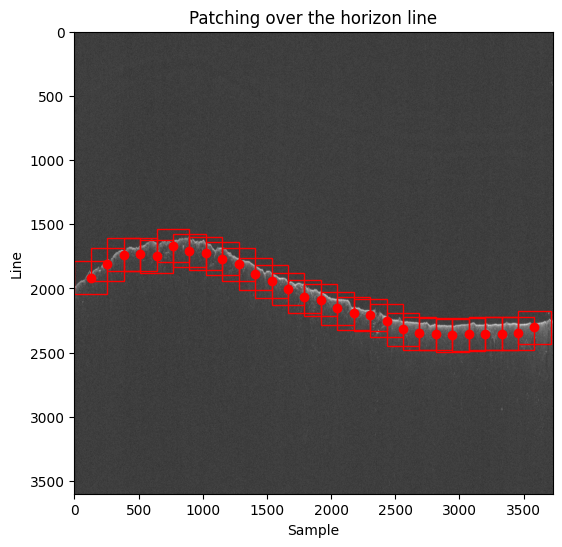
\includegraphics[width=\linewidth]{images/example_plots/ID_01970402/patching_example}
    \caption{Surface-aware patch extraction of sample with ID 01970402. Red markers indicate center of the box; colored boxes show extracted overlapping patches (28 total, 50\% overlap).}
    \label{fig:patch_extraction_column4160}
\end{figure}

To address these issues, a custom \textbf{Surface-Aware Patch Extraction} algorithm was implemented (executed via the \texttt{process.py} script, corresponding to the workflow in Block 2 of Figure~\ref{fig:system_architecture2}).
This strategy extracts square patches (fixed size $H \times W$, e.g., $128 \times 128$) focused specifically on the scientifically relevant subsurface regions.

The extraction procedure consists of four steps:
\begin{itemize}
    \item automated peak-finding identifies the surface reflection horizon across the azimuth dimension.
    \item a dynamic bounding box extracts a square patch (e.g., $128 \times 128$ pixels) below the top edge, capturing the relevant subsurface regions while rejecting non-informative atmospheric returns.
    \item verlapping patches are drawn with a 50\% stride ($W/2$), ensuring complete coverage and local redundancy.
    \item irregular binary structures are heuristically reconstructed or discarded, while extreme specular outliers are mitigated via robust Min-Max normalization (using the 1st and 99th percentiles) rather than explicit patch rejection.
\end{itemize}
Applied to Elysium Planitia observations, this pipeline yields $\sim$50k training patches while concentrating computational resources on signal-rich regions.

\begin{figure}[htbp]
    \centering
    \begin{subfigure}{\textwidth}
        \centering
        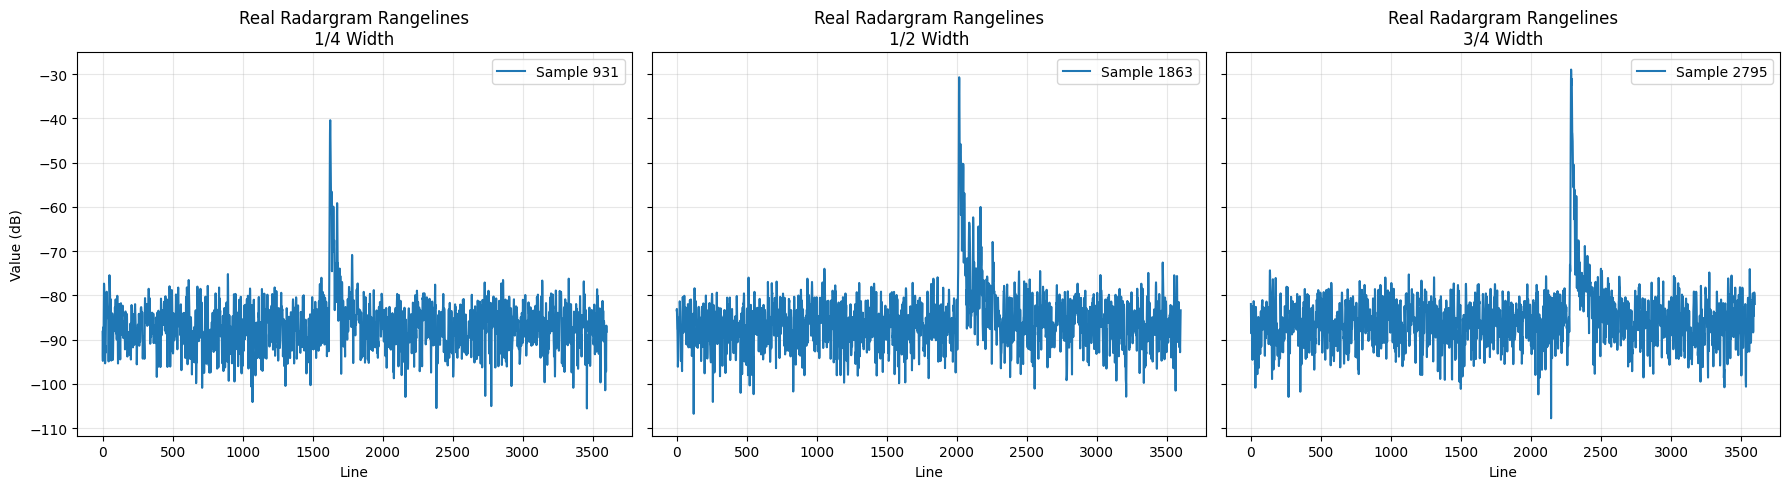
\includegraphics[width=\textwidth]{images/example_plots/ID_01970402/rangelines_real_db}
        \caption{Rangelines plotted in decibel (dB) scale. The profiles correspond to 0.25, 0.50, and 0.75 of the image width. A pronounced surface reflection is observed at approximately $-30$ to $-40$\,dB, whereas the majority of the signal is dominated by thermal noise around $-100$\,dB, illustrating sparse information density.}
        \label{fig:rangeline_sparse_density_db}
    \end{subfigure}
    
    \vspace{0.5em}
    
    \begin{subfigure}{\textwidth}
        \centering
        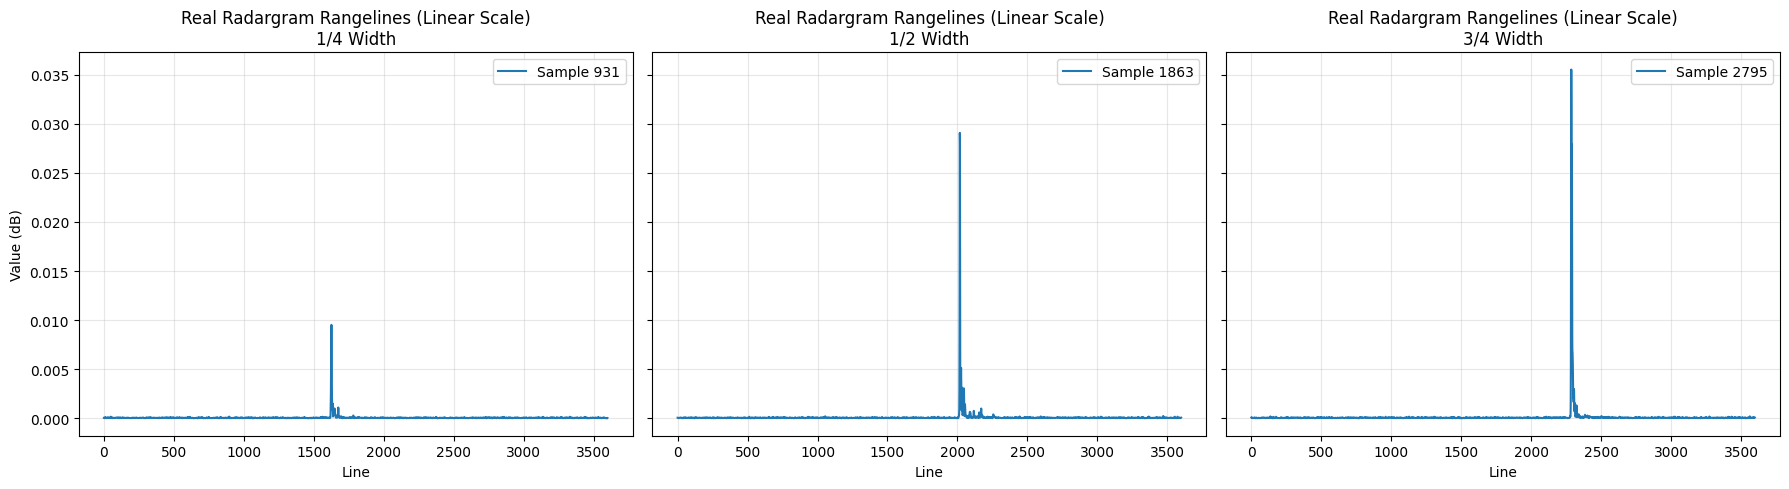
\includegraphics[width=\textwidth]{images/example_plots/ID_01970402/rangelines_real_linear}
        \caption{The same rangelines represented on a linear amplitude scale. The contrast between the surface reflection and the background noise becomes more pronounced, highlighting the large dynamic range of the signal.}
        \label{fig:rangeline_sparse_density_linear}
    \end{subfigure}
    
    \caption{Comparison of representative rangelines extracted at 0.25, 0.50, and 0.75 of the image width, shown in (a) logarithmic (dB) and (b) linear amplitude scales. The logarithmic representation emphasizes the noise floor and relative signal levels, while the linear representation accentuates the dominance of the surface reflection, demonstrating the sparse distribution of high-amplitude information within the scene.}
    \label{fig:rangeline_sparse_density}
\end{figure}

\subsection{Logarithmic Scaling and Dynamic Range Compression}
Radar signals are characterized by an extremely wide dynamic range, where the power of reflected echoes can span several orders of magnitude.
The specular reflection from the Martian surface often exhibits power levels millions of times greater than the faint dielectric contrasts of subsurface layers or the thermal noise floor.
If processed on a raw linear scale, these subtle subsurface features, which represent the primary targets of the present investigation, would be effectively invisible, quantized to the lowest values in a standard floating-point definition or lost entirely in the lower bits of an image format.

To address this, before patch extraction the first step in the pre-processing pipeline is the conversion of the linear power values, $P_{linear}$, into a logarithmic scale using the decibel (dB) unit.
This transformation is defined by the following equation:
$$ P_{dB} = 10 \log_{10}(P_{linear} + \epsilon) $$
where $\epsilon$ is a strictly positive infinitesimal constant (e.g., $10^{-13}$) to ensure numerical stability when $P_{linear} = 0$.

\subsection{Min-Max Normalization and Outlier Handling}
\label{subsec:minmax_normalization}
Deep learning models, particularly Generative Adversarial Networks (GANs), require input data to be normalized within a specific, bounded range to ensure stable gradient propagation.
The activation functions utilized in the generator (specifically the hyperbolic tangent, $\tanh$) and the discriminator typically operate most effectively when inputs are centered around zero with unit variance, or bounded within $[-1, 1]$.

In this framework, we adopt a Min-Max normalization strategy to rescale the decibel specifications to the $[-1, 1]$ interval. The transformation is given by:
\[ 
P_{norm} = 2 \frac{P_{dB} - v_{min}}{v_{max} - v_{min}} - 1 
\]
where $v_{min}$ and $v_{max}$ represent the global minimum and maximum power values observed across the entire training dataset.
It is crucial to note the statistical implications of this approach in the context of radar data.
Unlike natural images, where pixel values are naturally bounded (e.g., 0-255), radar power is theoretically unbounded.
In practice, coherent noise artifacts or specular reflections from orbital positioning maneuvers can produce "outliers" with anomalously high energy.
If $v_{max}$ is determined solely by the single brightest pixel in the entire dataset, a single artifact could stretch the normalization range excessively.
This would compress the vast majority of meaningful geological data into a tiny fraction of the $[-1, 1]$ range (e.g., $[-1, -0.9]$), effectively destroying the contrast required for the network to learn textures.
To mitigate this risk, our implementation calculates $v_{min}$ and $v_{max}$ using the 1st and 99th percentiles of the data distribution across the entire dataset.
This robust statistical approach ensures that the normalization range is determined by the geological signal rather than by transient instrument anomalies.

\begin{figure}[htbp]
    \centering
    \begin{subfigure}{\textwidth}
        \centering
        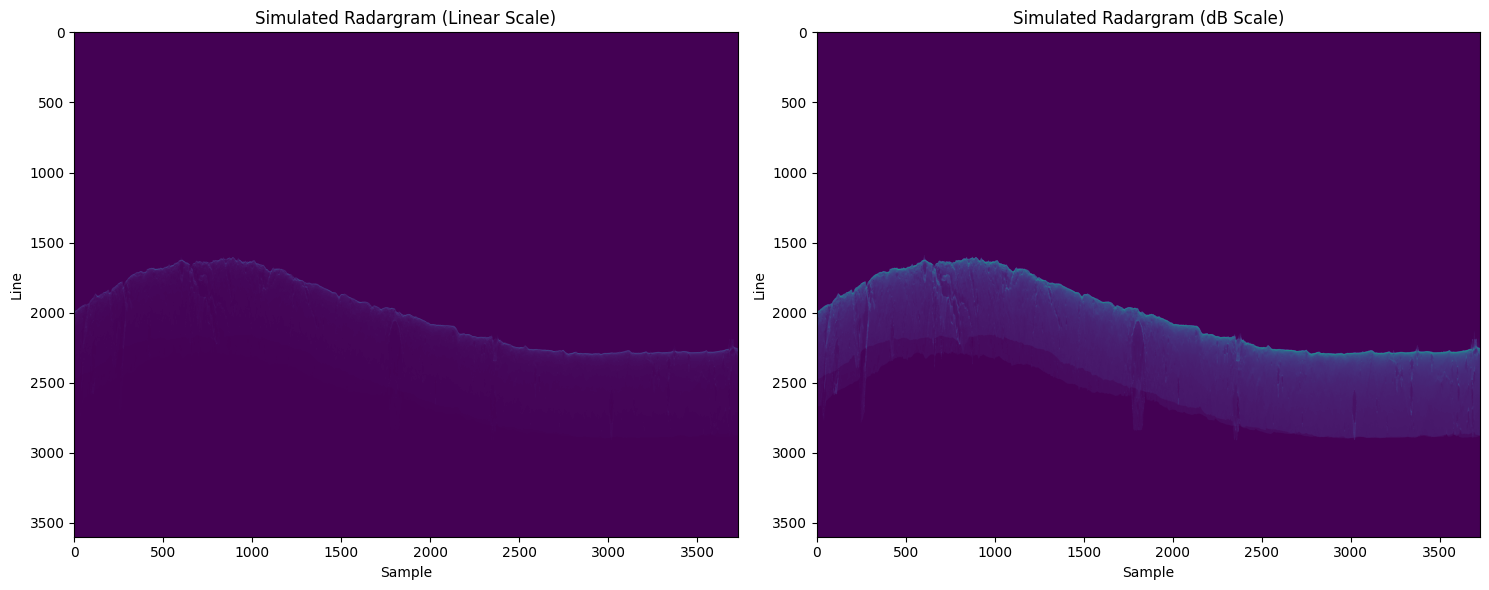
\includegraphics[width=\textwidth]{images/example_plots/ID_01970402/linear_vs_db_sim_RGB}
        \caption{Comparison using simulated SHARAD data. The left image shows the data in linear power scale; the right image in dB scale.}
        \label{fig:log_scaling_sim}
    \end{subfigure}
    
    \vspace{0.5em}
    
    \begin{subfigure}{\textwidth}
        \centering
        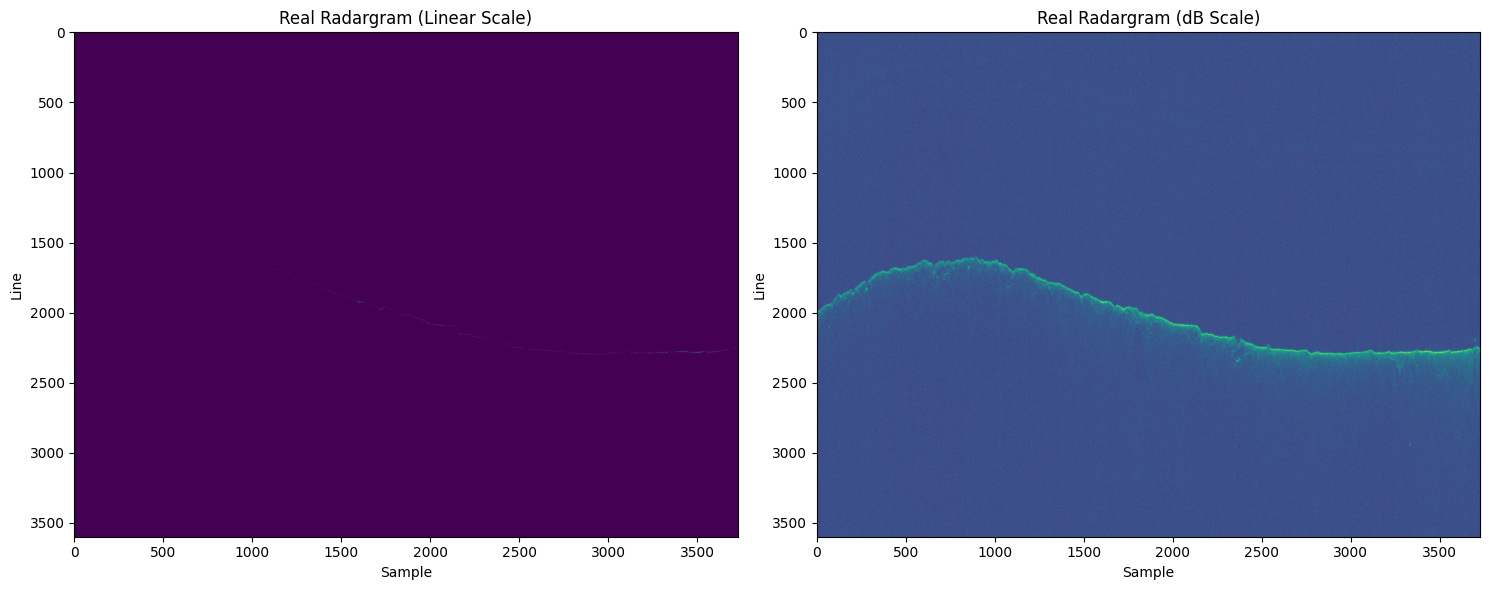
\includegraphics[width=\textwidth]{images/example_plots/ID_01970402/linear_vs_db_real_RGB}
        \caption{Comparison using real SHARAD data. The left image shows the data in linear power scale; the right image in dB scale.}
        \label{fig:log_scaling_real}
    \end{subfigure}
    
    \caption{Comparison of real and simulated SHARAD radargrams, each presented in (left) linear power scale and (right) logarithmic (dB) scale. (a) shows simulated data, (b) shows real data. For both, the linear plots are rendered using a dynamic range normalization (such as a median-based approach common in visualization libraries), causing the high-intensity surface reflection to be completely obscured by the statistical dominance of low-power subsurface and atmospheric returns. In the linear plot of the real data (b), the surface is invisible, while in the simulated data (a) it is only faintly visible. The dB transformation effectively compresses the dynamic range, providing numerical and perceptual accessibility to low-power geological features and a useful range for all information within the scene.}
    \label{fig:log_scaling_comparison}
\end{figure}

\subsection{Choice of the Data Normalization Strategy}
\label{subsec:ablation_normalization_study}
To justify the pre-processing decisions detailed in the previous subsections, we conducted an ablation study to compare three normalization approaches and their impact on the GAN's ability to generate realistic subsurface textures.
We recall that, unlike standard RGB images, radar data represents echo power with a potentially infinite dynamic range.

\subsubsection{Tested Approaches}
\begin{enumerate}
    \item \textbf{Method A: Linear Min-Max (Naive)}
    $$ x_{norm} = \frac{x - x_{min}}{x_{max} - x_{min}} $$
    Here, the raw power values are scaled linearly to [0, 1].
    
    \item \textbf{Method B: Z-Score Standardization}
    $$ x_{norm} = \frac{x - \mu}{\sigma} $$
    This centers the data around 0 with unit variance, common in many deep learning tasks.
    
    \item \textbf{Method C: Logarithmic Scaling + Min-Max (Proposed)}
    $$ x_{dB} = 10 \log_{10}(x + \epsilon) $$
    $$ x_{norm} = \frac{x_{dB} - \min(x_{dB})}{\max(x_{dB}) - \min(x_{dB})} $$
    The data is first converted to decibels (dB) to compress the dynamic range, and then scaled to $[-1, 1]$.
\end{enumerate}

\subsubsection{Results and Discussion}
The experiments revealed drastic differences in the quality of the learned distributions:

\begin{itemize}
    \item \textbf{Effect of Linear Scaling (Method A):} Radar data is dominated by the strong surface reflection, which can be orders of magnitude stronger than subsurface echoes. When using linear scaling, the surface peak sets the $x_{max}$ to a very high value, causing all faint subsurface features to be compressed into a tiny range near zero. Visually, the radargrams appeared almost black with a single white line (the surface). GANs trained on this data failed completely, learning only to generate a black background.
    \item \textbf{Effect of Z-Score (Method B):} While better than linear scaling, Z-score does not bound the data to a fixed range (e.g., $[-1, 1]$). Outliers (strong reflections) resulted in extreme values that pushed the \texttt{tanh} activation function into its saturation regions, leading to unstable training. This was primarily because the logarithmic transformation was not applied in this case, leading to ultimately worse performance than Method C.
    \item \textbf{Success of Logarithmic Scaling (Method C):} The logarithmic transformation naturally aligns with the physics of wave attenuation, compressing the orders of magnitude of power difference into a linear decibel scale. When combined with Min-Max scaling to $[-1, 1]$, it provided the optimal input for the network. The GAN successfully learned to distinguish and reproduce both the strong surface reflection and the delicate subsurface textures, as we will show in Chapter~\ref{cha:results}.
\end{itemize}

This study confirms that logarithmic pre-processing is not just an enhancement but a strict requirement for the convergence of GANs on radar sounding data.
We believe this is the driver of the success of Method C and it may also be applied to methods A and B.

\subsection{Surface Tracking Algorithm}
After normalizing the data, we perform a surface extraction process.
It is defined in the project's codebase (specifically \texttt{src/dataset/processing.py}), and uses an intelligent sliding window approach that adapts to the topography of the Martian surface.
For a given column $x$ in the radargram $R$, the algorithm identifies the surface horizon $y_{surf}$ as the index of the maximum signal intensity:
$$ y_{surf}(x) = \arg\max_j R(j, x) $$

A bounding box is then calculated to define the patch boundaries.
The vertical position of the box is not fixed but dynamically adjusted based on the local topography within the window width $W$.
The algorithm computes the minimum ($y_{min}$) and maximum ($y_{max}$) horizon depth within the interval $[x - W/2, x + W/2]$ to determine a \texttt{top\_edge}.
From this upper boundary, the bounding box extends downwards by a fixed patch height $H$.
This parameter $H$ is crucial as it defines the maximum depth of the geological context provided to the model.
The resulting extracted patch has fixed dimensions of $W \times H$, a design that ensures the surface interface is always contained within the upper portion of the patch, while maximizing the inclusion of the subsurface layers below it.

\begin{figure}[htbp]
    \centering
    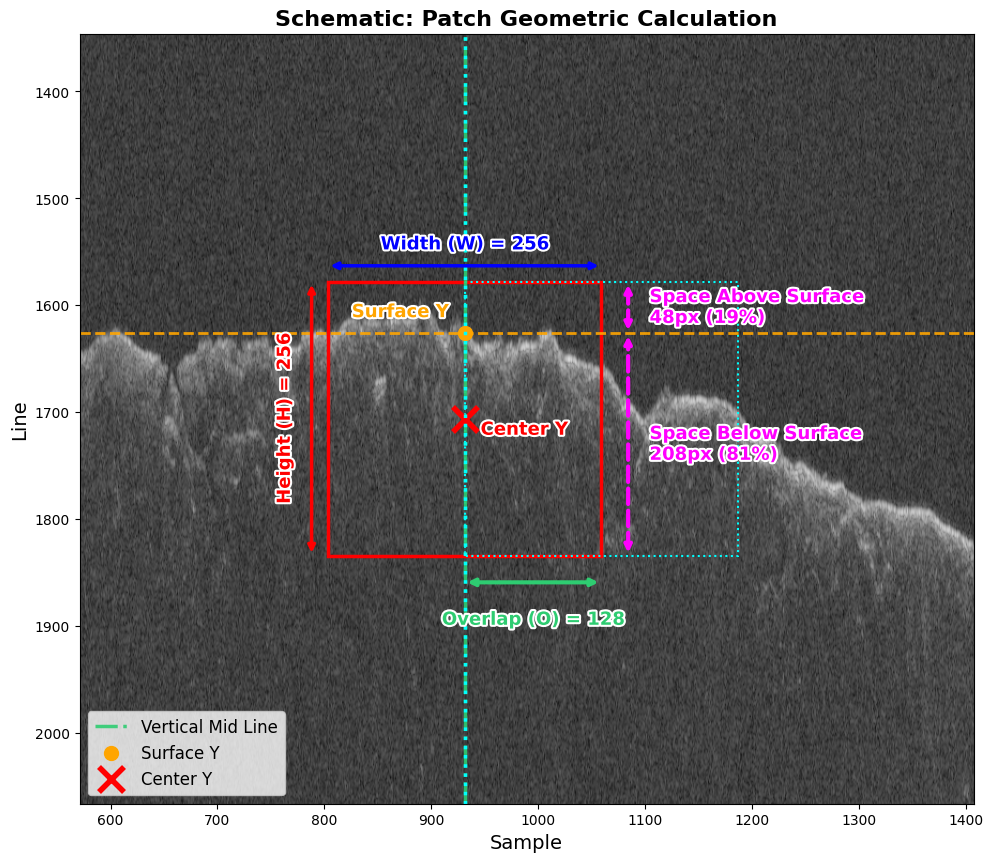
\includegraphics[width=0.8\textwidth]{images/example_plots/ID_01970402/patch_schematic}
    \caption{Illustration of the sliding window and patching mechanism on a Martian radargram. The red line represents the tracked surface $y_{surf}$. The highlighted bounding box demonstrates the extraction of a single patch of width $W$ and height $H$, starting from the dynamically adjusted \texttt{top\_edge}.}
    \label{fig:patching_logic}
\end{figure}

\subsection{Sliding Window and Overlap}
To prevent data loss at the boundaries of the patches---a common issue known as the \enquote{edge effect} where predictions degrade near the image borders---the patches are extracted with a significant overlap.
The stride $S$ of the sliding window is defined as:
$$ S = W - O $$
where $O$ is the overlap parameter (typically $W/2$).
This ensures that every geological feature appears in multiple patches, often centered in at least one, allowing the network to learn robust features invariant to their relative position in the input window.
Importantly, $O$ is not chosen too large to prevent samples from being too correlated with each other while still maintaining a reasonable number of independent samples for training.

\subsubsection{Handling Irregular Data Structures}
A significant practical challenge in the pre-processing pipeline was the intrinsic inconsistency of the raw PDS data products.
Although the SHARAD archive follows a well-defined standard, a non-negligible fraction of files exhibits irregularities in the binary layout, such as flattened arrays, non-standard padding, or truncated range lines.
If handled naively, these cases would either cause hard failures in the import stage or be silently discarded, effectively reducing the usable volume of the training dataset and biasing the statistics towards only the \enquote{cleanest} acquisitions.

To mitigate this issue, a custom heuristic procedure, implemented in the \texttt{handle\_irregular\_data} routine, was developed to reconstruct two-dimensional radargrams from such irregular binary arrays.
The algorithm operates in a multi-stage fashion.
First, it performs a consistency check against known SHARAD acquisition parameters by comparing the raw vector length with common radargram dimensions (e.g., $3600$ range samples per line) and their integer factors, noting that data in the PDS Object Description Exchange (ODE) is organized as a continuous stream of bytes rather than pre-formed 2D arrays.
When a direct reshape to $(N_{\text{range}}, N_{\text{azimuth}})$ is not possible, the routine estimates a plausible number of range samples by taking the median length over a local batch of products belonging to the same orbit or observation segment, under the assumption that their acquisition settings are identical.

In more pathological cases, the algorithm falls back to a brute-force factorization strategy: given a one-dimensional array of length $L$, it enumerates factor pairs $(n_r, n_a)$ such that $n_r \times n_a = L$ and favors configurations where $n_r$ is close to typical SHARAD values (e.g., $n_r \approx 3600$) while $n_a$ remains within a reasonable range for along-track extent.
Candidate reshapes are then validated by simple sanity checks on the resulting 2D image, such as verifying that the maximum power response lies near the expected surface region and that no entire rows or columns are saturated or identically zero.

If at least one configuration passes these heuristic tests, the corresponding reshaped radargram is accepted and forwarded to the subsequent logarithmic scaling and normalization stages described above; otherwise, the product is flagged as irrecoverable and excluded.
This robust handling of irregular data structures prevents the training pipeline from being halted by corrupted or non-standard PDS products and maximizes the amount of information that can be recovered from the archive, thereby increasing the statistical diversity and coverage of the final training set.

